
% This LaTeX was auto-generated from MATLAB code.
% To make changes, update the MATLAB code and republish this document.

\documentclass{article}
\usepackage{graphicx}
\usepackage{color}

\sloppy
\definecolor{lightgray}{gray}{0.5}
\setlength{\parindent}{0pt}

\begin{document}

    
    

\section*{8. Convergence for analytic functions}

\begin{verbatim}
ATAPformats
\end{verbatim}
\begin{par}

Suppose $f$ is not just $k$ times differentiable but infinitely
differentiable and in fact analytic on $[-1,1]$.  (Recall that this means
that for any $s\in [-1,1]$, $f$ has a Taylor series about $s$ that
converges to $f$ in a neighborhood of $s$.)  Then without any further
assumptions we may conclude that the Chebyshev projections and
interpolants converge {\bf geometrically}, that is, at the rate
$O(C^{-n})$ for some constant $C>1$.  This means the errors will look
like straight lines (or better) on a semilog scale rather than a loglog
scale. This kind of connection was first announced by Bernstein in 1911,
who showed that the best approximations to a function $f$ on $[-1,1]$
converge geometrically as $n\to\infty$ if and only if $f$ is analytic
[Bernstein 1911 \& 1912{\sc b}].

\end{par} \vspace{1em}
\begin{par}
For example, for Chebyshev interpolants of the function $(1+25x^2)^{-1}$, known as the \textit{Runge function} (Chapter 13), we get steady geometric convergence down to the level of rounding errors:
\end{par} \vspace{1em}
\begin{par}
 \vskip -2em 
\end{par} \vspace{1em}
\begin{verbatim}
x = chebfun('x'); f = 1./(1+25*x.^2); nn = 0:10:200; ee = 0*nn;
for j = 1:length(nn)
    n = nn(j); fn = chebfun(f,n+1); ee(j) = norm(f-fn,inf);
end
hold off, semilogy(nn,ee,'.'), grid on, axis([0 200 1e-17 10])
FS = 'fontsize';
title(['Geometric convergence of Chebyshev ' ...
      ' interpolants -- analytic function'],FS,9)
\end{verbatim}

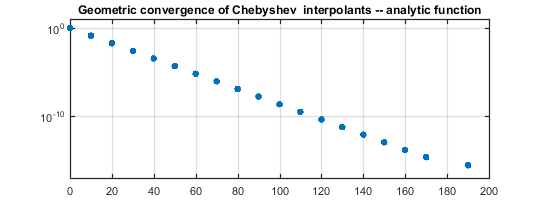
\includegraphics [width=4in]{chap8_01.png}
\begin{par}
 \vskip 1pt 
\end{par} \vspace{1em}
\begin{par}
If $f$ is analytic not just on $[-1,1]$ but in the whole complex plane---such a function is said to be \textit{entire}---then the convergence is even faster than geometric. Here, for the function $\cos(20x)$, the dots are not approaching a fixed straight line but a curve that gets steeper as $n$ increases, until rounding errors cut off the progress.
\end{par} \vspace{1em}
\begin{par}
 \vskip -2em 
\end{par} \vspace{1em}
\begin{verbatim}
f = cos(20*x); nn = 0:2:60; ee = 0*nn;
for j = 1:length(nn)
    n = nn(j); fn = chebfun(f,n+1); ee(j) = norm(f-fn,inf);
end
semilogy(nn,ee,'.'), grid on, axis([0 60 1e-16 100])
title('Convergence of Chebyshev interpolants -- entire function',FS,9)
\end{verbatim}

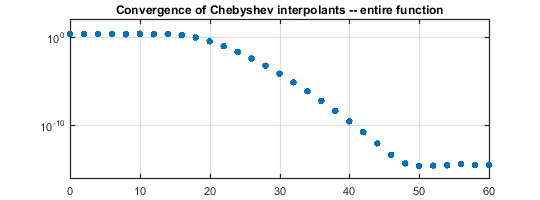
\includegraphics [width=4in]{chap8_02.png}
\begin{par}
 \vskip 1pt 
\end{par} \vspace{1em}
\begin{par}

There are elegant theorems that explain these effects. If $f$ is analytic
on $[-1,1]$, then it can be analytically continued to a neighborhood of
$[-1,1]$ in the complex plane.  (The idea of analytic continuation is
explained in complex variables textbooks; see also Chapter 28.)  The
bigger the neighborhood, the faster the convergence. In particular, for
polynomial approximations, the neighborhoods that matter are the regions
in the complex plane bounded by ellipses with foci at $-1$ and $1$,
known as {\em Bernstein ellipses}
[Bernstein 1912{\sc b}, 1912{\sc c} \&
1914{\sc a}]. It is easy to plot these curves: pick a number $\rho>1$
and plot the image in the complex $x$-plane of the circle of radius
$\rho$ in the $z$-plane under the Joukowsky map $x = (z+z^{-1})/2$.  We
let $E_\rho$ denote the open region bounded by this ellipse. Here, for
example, are the Bernstein ellipses corresponding to the parameters $\rho
= 1.1,1.2,\dots,2$:

\end{par} \vspace{1em}
\begin{par}
 \vskip -2em 
\end{par} \vspace{1em}
\begin{verbatim}
z = exp(2i*pi*x);
for rho = 1.1:0.1:2
    e = (rho*z+(rho*z).^(-1))/2; plot(e), hold on
end
ylim([-.9 .9]), axis equal
title('Bernstein ellipses for \rho = 1.1, 1.2, ..., 2',FS,9)
\end{verbatim}

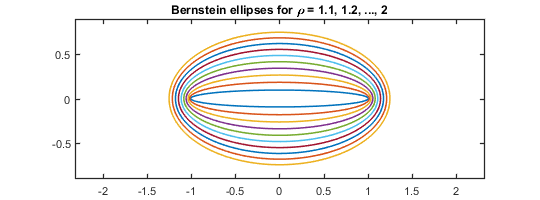
\includegraphics [width=4in]{chap8_03.png}
\begin{par}
 \vskip 1pt 
\end{par} \vspace{1em}
\begin{par}
It is not hard to verify that the length of the semimajor axis of $E_\rho$ plus the length of the semiminor axis is equal to $\rho$ (Exercise 8.1).
\end{par} \vspace{1em}
\begin{par}
Here is the basic bound on Chebyshev coefficients of analytic functions from which many other things follow.  It first appeared in Section 61 of [Bernstein 1912b].
\end{par} \vspace{1em}
\begin{par}
 \em
{\bf Theorem 8.1. Chebyshev coefficients of analytic functions.} Let a
function $f$ analytic in $[-1,1]$ be analytically continuable to the open
Bernstein ellipse $E_\rho$, where it satisfies $|f(x)|\le M$ for some
$M$.  Then its Chebyshev coefficients satisfy $|a_0| \le M$ and
$$ | a_k | \le 2M\rho^{-k},\quad k\ge 1. \eqno (8.1) $$
\vspace{0em} 
\end{par} \vspace{1em}
\begin{par}
\textit{Proof.} As in the proofs of Theorems 3.1, 4.1, and 7.1, we make use of the transplantation from $f(x)$ and $T_k(x)$ on $[-1,1]$ in the $x$-plane to $F(z)$ and $(z^k + z^{-k})/2$ on the unit circle in the $z$-plane, with $x = (z+z^{-1})/2$ and $F(z) = F(z^{-1}) = f(x)$.  The ellipse $E_\rho$ in the $x$-plane corresponds under this formula in a 1-to-2 fashion to the annulus $\rho^{-1} < |z| < \rho$ in the $z$-plane.  By this we mean that for each $x$ in $E_\rho\backslash [-1,1]$ there are two corresponding values of $z$ which are inverses of one another, and both the circles $|z|=\rho$ and $|z|=\rho^{-1}$ map onto the ellipse itself. (We can no longer use the formula $x = \hbox{Re}\,z$, which is valid only for $|z|=1$.) The first thing to note is that if $f$ is analytic in the ellipse, then $F$ is analytic in the annulus since it is the composition of the two analytic functions $z \mapsto (z+z^{-1})/2$ and $x \mapsto f(x)$. Now we make use of the contour integral formula (3.12), $$ a_k  = {1\over\pi i}\int_{|z|=1}z^{-1-k}F(z)\,dz, $$ with $\pi i$ replaced by $2\pi i$ for $k=0$. Suppose for a moment that $F$ is analytic not just in the annulus but in its closure $\rho^{-1} \le |z| \le \rho$. Then we can expand the contour to $|z|=\rho$ without changing the value of the integral, giving $$ a_k= {1\over\pi i}\int_{|z|=\rho}z^{-1-k}F(z)\,dz, $$ again with $\pi i$ replaced by $2\pi i$ for $k=0$. Since the circumference is $2\pi \rho$ and $|F(z)| \le M$, the required bound now follows from an elementary estimate. If $F$ is analytic only in the open annulus, we can move the contour to $|z|=s$ for any $s<\rho$, leading to the same bound for any $s<\rho$ and hence also for $s=\rho$. $~\hbox{\vrule width 2.5pt depth 2.5 pt height 3.5 pt}$
\end{par} \vspace{1em}
\begin{par}
Here are two of the consequences of Theorem 8.1.  Equation (8.2) first appeared in [Bernstein 1912b, Sec. 61]. I do not know where equation (8.3) may have appeared, though similar slightly weaker bounds can be found in (4.13) and (4.16) of [Tadmor 1986]. For a generalization of (8.3) to interpolation in other point sets with the same asymptotic distribution as Chebyshev points, see Theorem 12.1.
\end{par} \vspace{1em}
\begin{par}
 \em
{\bf Theorem 8.2. Convergence for analytic functions.}
If $f$ has the properties of Theorem $8.1$, then for
each $n\ge 0$ its Chebyshev projections satisfy
$$ \| f - f_n \| \le {2M\rho^{-n}\over \rho - 1} \eqno (8.2) $$
and its Chebyshev interpolants satisfy
$$ \| f - p_n \| \le {4M\rho^{-n}\over \rho - 1}. \eqno (8.3) $$
\vspace{-1.5em} 
\end{par} \vspace{1em}
\begin{par}
\textit{Proof.}  Equation (8.2) follows from Theorem 8.1 and (4.8), and (8.3) follows from Theorem 8.1 and (4.9). $~\hbox{\vrule width 2.5pt depth 2.5 pt height 3.5 pt}$
\end{par} \vspace{1em}
\begin{par}
We can apply Theorem 8.2 directly if $f$ is analytic and bounded in $E_\rho$. If it is analytic but unbounded in $E_\rho$, then it will be analytic and bounded in $E_s$ for any $s<\rho$, so we still get convergence at the rate $O(s^{-n})$ for any $s<\rho$. If it is unbounded in $E_\rho$ but the only singularities on the ellipse are simple poles, then we get convergence at the rate $O(\kern .5pt\rho^{-n})$ after all (Exercise 8.15).
\end{par} \vspace{1em}
\begin{par}

Before applying Theorem 8.2 to a couple of examples, it will be
convenient to note formulas for $\rho$ in two common special cases.
Suppose $f$ has its first singularity at a real value $x_0 = \pm \alpha$
for some $\alpha>1$. Then the corresponding ellipse parameter is
$$ \rho = \alpha + \sqrt{\alpha^2-1} \quad \hbox{(real singularity at $x = \pm \alpha$).}
\eqno (8.4) $$
Or suppose that the first singularity is at the pure imaginary value
$x_0 = \pm i\beta$ for some $\beta>0$.  Then we have
$$ \rho = \beta + \sqrt{\beta^2+1} \quad \hbox{(imaginary singularity at $x = \pm i\beta$).}
\eqno (8.5) $$

\end{par} \vspace{1em}
\begin{par}
For example, the Runge function $(1+25x^2)^{-1}$ considered above has poles at $\pm i/5$.  By (8.5), the corresponding value of $\rho$ is $(1+\sqrt{26}\kern .7pt )/5 \approx 1.220$, and the errors in Chebyshev interpolation match this rate beautifully:
\end{par} \vspace{1em}
\begin{par}
 \vskip -2em 
\end{par} \vspace{1em}
\begin{verbatim}
f = 1./(1+25*x.^2); nn = 0:10:200; ee = 0*nn;
for j = 1:length(nn)
    n = nn(j); fn = chebfun(f,n+1); ee(j) = norm(f-fn,inf);
end
rho = (1+sqrt(26))/5;
hold off, semilogy(nn,rho.^(-nn),'-r')
hold on, semilogy(nn,ee,'.'), grid on, axis([0 200 1e-17 10])
title('Geometric convergence for the Runge function',FS,9)
\end{verbatim}

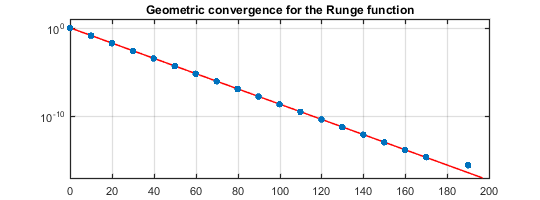
\includegraphics [width=4in]{chap8_04.png}
\begin{par}
 \vskip 1pt 
\end{par} \vspace{1em}
\begin{par}
Here is a more extreme but entirely analogous example: $\tanh(50 \pi x)$, with poles at $\pm 0.01i$.  These poles are so close to $[-1,1]$ that the convergence is much slower, but it is still robust.  The only difference in this code segment is that \texttt{norm(f-fn,inf)}, a relatively slow Chebfun operation that depends on finding zeros of the derivative of \texttt{f-fn}, has been replaced by the default 2-norm \texttt{norm(f-fn)}, which is quick.  This makes little difference to the figure, as the exponential decay rates are the same.  (In the $\infty$-norm, the dots in the figure would appear just above the red line instead of just below it.)
\end{par} \vspace{1em}
\begin{par}
 \vskip -2em 
\end{par} \vspace{1em}
\begin{verbatim}
f = tanh(50*pi*x); nn = 0:200:4000; ee = 0*nn;
for j = 1:length(nn)
    n = nn(j); fn = chebfun(f,n+1); ee(j) = norm(f-fn);
end
rho = (1+sqrt(10001))/100;
hold off, semilogy(nn,rho.^(-nn),'-r')
hold on, semilogy(nn,ee,'.')
grid on, axis([0 4000 1e-16 10])
title(['Geometric convergence for a function ' ...
       'analytic in a narrow region'],FS,9)
\end{verbatim}

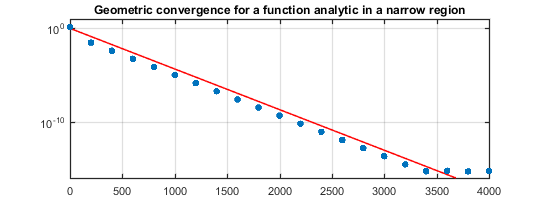
\includegraphics [width=4in]{chap8_05.png}
\begin{par}
 \vskip 1pt 
\end{par} \vspace{1em}
\begin{par}
For an example with a real singularity, the function $\sqrt{2-x}$ has a branch point at $x=2$, corresponding by (8.4) to $\rho = 2+\sqrt{3}$. Again we see a good match, with the curve gradually bending over to the expected slope as $n\to\infty$.
\end{par} \vspace{1em}
\begin{par}
 \vskip -2em 
\end{par} \vspace{1em}
\begin{verbatim}
f = sqrt(2-x);
nn = 0:30; ee = 0*nn;
for j = 1:length(nn)
    n = nn(j); fn = chebfun(f,n+1); ee(j) = norm(f-fn,inf);
end
rho = 2+sqrt(3);
hold off, semilogy(nn,rho.^(-nn),'-r')
hold on, semilogy(nn,ee,'.')
grid on, axis([0 30 1e-17 10])
title(['Geometric convergence for an analytic ' ...
       'function with a branch point'],FS,9)
\end{verbatim}

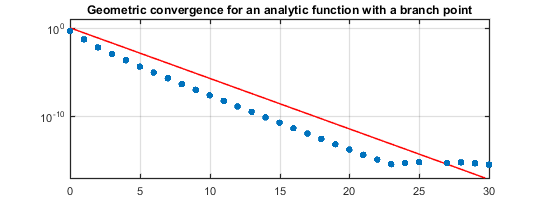
\includegraphics [width=4in]{chap8_06.png}
\begin{par}
 \vskip 1pt 
\end{par} \vspace{1em}
\begin{par}
We now derive an elegant converse of Theorem 8.2, also due to Bernstein [1912b, Section 9].  The converse is not quite exact: Theorem 8.2 assumes analyticity and boundedness in $E_\rho$, whereas the conclusion of Theorem 8.3 is analyticity but not necessarily boundedness (Exercise 8.15).
\end{par} \vspace{1em}
\begin{par}
\textbf{Theorem 8.3. Converse of Theorem 8.2.} \textit{Suppose $f$ is a function on $[-1,1]$ for which there exist polynomial approximations $\{q_n\}$ satisfying} $$   \| f - q_n \| \le C\rho^{-n}, \quad n\ge 0  $$ \textit{for some constants $\rho>1$ and $C>0$. Then $f$ can be analytically continued to an analytic function in the open Bernstein ellipse} $E_{\rho}$.
\end{par} \vspace{1em}
\begin{par}
\textit{Proof.}  The assumption implies that the polynomials $\{q_n\}$ satisfy $\|q_n-q_{n-1}\|\le 2\kern .7pt C\kern .4pt \rho^{1-n}$ on $[-1,1]$. Since $q_n-q_{n-1}\in {\cal P}_n$, it can be shown that this implies $\|q_n - q_{n-1}\|_{E_s} \le 2\, C s^n \rho^{1-n} $ for any $s>1$, where $\|\cdot\|_{E_s}$ is the supremum norm on the $s$-ellipse $E_s$. (This estimate is one of \textit{Bernstein's inequalities,} from Section 9 of [Bernstein 1912b]; see Exercise 8.6.) For $s<\rho$, this gives us a representation for $f$ in $E_s$ as a series of analytic functions, $$ f = q_0 + (q_1-q_0) + (q_2-q_1) + \cdots , $$ which is uniformly convergent according to the Weierstrass M-test. According to another well-known theorem of Weierstrass, this implies that the limit is a bounded analytic function [Ahlfors 1953, Markushevich 1985]. Since this is true for any $s<\rho$, the analyticity applies throughout $E_\rho$. $~\hbox{\vrule width 2.5pt depth 2.5 pt height 3.5 pt}$
\end{par} \vspace{1em}
\begin{par}
Note that Theorem 8.2 and 8.3 together establish a simple fact, sometimes known as \textit{Bernstein's theorem}: a function defined on $[-1,1]$ can be approximated by polynomials with geometric accuracy if and only if it is analytic.  (See also Exercise 8.11 and [Bagby \& Levenberg 1993].)
\end{par} \vspace{1em}
\begin{par}
The term ``Bernstein ellipse'' refers to any ellipse in the complex plane with foci $\{-1,1\}$, and if $f$ is a function analytic on $[-1,1]$, the bounds of Theorems 8.1 and 8.2 apply for any Bernstein ellipse inside which $f$ is analytic and bounded.  If there is a largest ellipse inside which $f$ is analytic, then one might choose to say that this was ``the'' Bernstein ellipse for $f$, but this might not always be the ellipse that gives the most useful bound, and if $f$ is entire, then there is no largest ellipse at all (Exercise 8.3).
\end{par} \vspace{1em}
\begin{par}
Chebfun computations, however, suggest a practical way to single out a special Bernstein ellipse associated with a given function $f$.  The \textit{Chebfun ellipse} for $f$ is the Bernstein ellipse whose parameter $\rho$ satisfies the condition $$ \rho^{-n} = \varepsilon, \eqno (8.6) $$ where $\varepsilon$ is the tolerance used by the Chebfun constructor (normally $2^{-52}$) and $n$ is the degree of the polynomial chosen by Chebfun to resolve $f$.  The command \texttt{chebellipseplot} plots these Chebfun ellipses. Thus for $f(x) = 1/(1+25x^2)$, for example, the Chebfun ellipse comes very close to passing through the poles at $\pm 0.2i$:
\end{par} \vspace{1em}
\begin{par}
 \vskip -2em 
\end{par} \vspace{1em}
\begin{verbatim}
f = chebfun('1./(1+25*x.^2)');
clf, chebellipseplot(f,'linewidth',1)
hold on, plot([.2i -.2i],'xr','markersize',12)
axis equal, ylim(.5*[-1 1]), grid on
title('Chebfun ellipse for 1/(1+25x^2)',FS,9)
\end{verbatim}

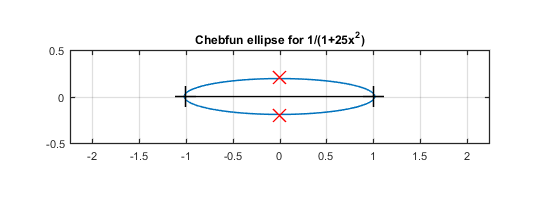
\includegraphics [width=4in]{chap8_07.png}
\begin{par}
 \vskip 1pt 
\end{par} \vspace{1em}
\begin{par}
For the entire function $f(x) = \exp(-200x^2)$, the Chebfun ellipse has much the same shape although now $f$ has no singularities:
\end{par} \vspace{1em}
\begin{par}
 \vskip -2em 
\end{par} \vspace{1em}
\begin{verbatim}
f = chebfun('exp(-200*x.^2)');
hold off, chebellipseplot(f,'linewidth',1)
axis equal, ylim(.5*[-1 1]), grid on
title('Chebfun ellipse for exp(-200x^2)',FS,9)
\end{verbatim}

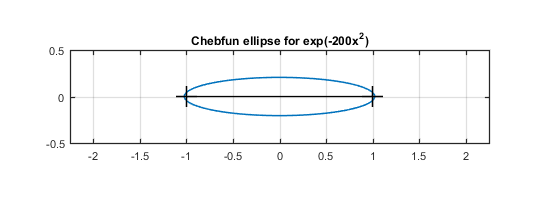
\includegraphics [width=4in]{chap8_08.png}
\begin{par}
 \vskip 1pt 
\end{par} \vspace{1em}
\begin{par}

\begin{displaymath}
\framebox[4.7in][c]{\parbox{4.5in}{\vspace{2pt}\sl
{\sc Summary of Chapter 8.} If $f$ is analytic, its Chebyshev
coefficients $\{a_k\}$ decrease geometrically.  In particular, if $f$ is
analytic with $|f(x)| \le M$ in the Bernstein $\rho$-ellipse about
$[-1,1]$, then $|a_k|\le 2M\rho^{-k}$.  It follows that the degree $n$
Chebyshev projection and interpolant of $f$ have accuracy
$O(M\rho^{-n})$.\vspace{2pt}}}
\end{displaymath}

\end{par} \vspace{1em}
\begin{par}
 \smallskip\small\parskip=2pt
{\bf Exercise 8.1.  Bernstein ellipses.} Verify that for any $\rho >1$,
the length of the
semiminor axis plus the length of the semimajor axis of the Bernstein
ellipse $E_\rho$ is equal to $\rho$.
\par
{\bf Exercise 8.2.  A Chebyshev series.}
With {\tt x = chebfun('x')}, execute the command
{\tt chebpolyplot(sin(100*(x-.1))+.01*tanh(20*x))}.  Explain the various
features of the resulting plot as quantitatively as you can.
\par
{\bf Exercise 8.3.  Interpolation of an entire function.}  The
function $f(x) = \exp(-x^2)$ is analytic throughout the complex $x$-plane,
so Theorem 8.2 can be applied for any
value of the parameter $\rho>1$.
Produce a semilog plot of $\|f-p_n\|$ as a function of $n$
together with lines corresponding to the upper bound of the theorem for
$\rho = 1.1, 1.2, 1.4, 2, 3, 5, 8$.  Be sure to use the
right value of $M$ in each case.  How well do your bounds fit the data?
\par
{\bf Exercise 8.4.  Convergence rates for different functions.}
Based on the theorems of this chapter, what can you say about
the convergence as $n\to\infty$ of the Chebyshev interpolants to
(a) $\tan(x)$,
(b) $\tanh(x)$,
(c) $\log((x+3)/4)/(x-1)$,
(d) $\int_{-1}^x \cos(t^2)\kern 1pt dt$,
(e) $\tan(\tan(x))$,
(f) $(1+x) \log(1+x)\,$?
In each case compare theoretical bounds with numerically computed
results.  Which is the case that converges much faster than the
theorems predict?  Can you speculate as to why?
\par
{\bf Exercise 8.5.  Accuracy of approximations in the complex plane.} Let
$p$ be the chebfun for $f(x) = \exp(-200x^2)$ and plot contour lines in
the complex $x$-plane corresponding to $|f(x) - p(x)| = 10^{-2}, 10^{-4},
\dots, 10^{-14}$.  How do these curves compare to the Bernstein ellipses
corresponding to parameters $\rho$ satisfying $\rho^{-n} = \varepsilon
\times \{ 10^2, 10^4, \dots , 10^{14}\}$, where $\varepsilon$ is the
Chebfun constructor tolerance $2^{-52}\kern 1pt$?
\par
{\bf Exercise 8.6.  Proof of Bernstein inequality.} Prove Bernstein's
inequality used in the proof of Theorem 8.3: if $p$ is a polynomial of
degree $d$, then $\|\kern .7pt p\|_{E_\rho} \le \rho^d \kern 1pt \|\kern
.7pt p\|$, where $\|\cdot \|_{E_\rho}$ is the $\infty$-norm over the
$\rho$-ellipse and $\|\cdot\|$ is the $\infty$-norm over $[-1,1]$. (Hint:
Show that if the branch cut is taken to be the unit interval $[-1,1]$,
the function $q(z) = p(z)/(z+(z^2-1)^{1/2})^d$ is analytic throughout the
region consisting of the complex plane plus the point $z=\infty$ minus
$[-1,1]$. Apply the maximum modulus principle.)
\par
{\bf Exercise 8.7.  Absolute value function.}
The function $|x-i|$ is analytic for $x\in [-1,1]$.
This means it can be analytically continued to an analytic
function $f(x)$ in a neighborhood of $[-1,1]$ in the complex $x$-plane.
The formula $|x-i|$ itself does not define an analytic function
in any complex neighborhood.  Find another formula for $f$ that does,
and use it to explain what singularities $f$ has in the complex plane.
\par
{\bf Exercise 8.8.  Chebyshev polynomials on the Bernstein ellipse.}
Show that for any $\rho>1$ and any $z$ on the boundary of the
ellipse $E_\rho$ in the complex $x$-plane,
$\lim_{n\to\infty} |T_n(x)|^{1/n} = \rho$.
\par
{\bf Exercise 8.9.  You can't judge smoothness by eye.}
Define $f(x) = 2+\sin(50x)$ and $g(x) = f(x)^{1.0001}$ and
construct chebfuns for these functions on $[-1,1]$.  What are
their lengths?  Explain this effect quantitatively
using the theorems of this chapter.
\par
{\bf Exercise 8.10.  Convergence of conjugate gradient iteration.}
Suppose we wish to approximate $f(x) = x^{-1}$ on the interval $[m,M]$
with $0 < m<M $. Show that for any $\kappa < M/m$, there exist
polynomials $p_n\in {\cal P}_n$ such that $\|f-p_n\| =
O((1+2/\sqrt\kappa\kern 1pt )^{-n})$ as $n\to\infty$, where $\|\cdot\|$
is the $\infty$-norm on $[m,M]$. This result is famous in numerical
linear algebra as providing an upper bound for the convergence of the
conjugate gradient iteration applied to a symmetric positive definite
system of equations $Ax=b$ with condition number $\kappa$. See Theorem
38.5 of [Trefethen \& Bau 1997].
\par
{\bf Exercise 8.11.  Bernstein's theorem.}
Show that the conclusion of Theorem 8.3 also holds if the hypothesis
is weakened to $\limsup_{n\to\infty}\|f-q_n\|^{1/n} \le \rho^{-1}$.
\par
{\bf Exercise 8.12. Resolution power of Chebyshev interpolants.}
The function $f_M(x) = \exp(-M^2x^2/2)$ has a spike of width $O(1/M)$
at $x=0$.  Let $n(M)$ be the degree of a chebfun for $f_M$.
(a) Determine the asymptotic behavior of $n(M)$ as $M\to\infty$ by
numerical experiments.
(b) Explain this result based on the theorems of this chapter.
\par
{\bf Exercise 8.13. Resolution power of Bernstein polynomials.}
Continuing the last exercise, now let $n(M)$ be the degree of
a Bernstein polynomial (6.1) needed to approximate $f_M$
to machine precision.  (For this discussion rescale (6.1) from
$[0,1]$ to $[-1,1]$.)
(a) Determine the asymptotic behavior of $n(M)$ as $M\to\infty$ by
numerical experiments.
(b) Explain this result, not necessarily rigorously.
\par
{\bf Exercise 8.14. Formulas for ellipse parameter.}
Derive (8.4) and (8.5).
\par
{\bf Exercise 8.15. Simple poles on the Bernstein ellipse.}
(a) Explain how equation (3.16)
illustrates that Theorem 8.3 is not an exact converse of Theorem 8.2.
(b) Let $f$ be analytic in the open Bernstein ellipse
region $E_\rho$ for some $\rho>1$ with the only singularities
on the ellipse itself being simple poles.  Show that
$\|f-f_n\|$ and $\|f-p_n\|$ are of size $O(\kern .5pt\rho^{-n})$ as $n\to\infty$.
\par 
\end{par} \vspace{1em}



\end{document}
    
